
% !TEX root = ../main.tex

% Local Variables:
% TeX-master: "../main"
% End:
% chktex-file 26

%%%%%%%%%%%%%%%%%%%%%%%%%%%%%%% Header %%%%%%%%%%%%%%%%%%%%%%%%%%%%%%%%%%%%%%%%%%%%
\begin{minipage}[l]{0.42\textwidth}
    
\includegraphics[width=1\textwidth]{img/logo-UNAMBA.png}
\end{minipage}
\hfill
\begin{minipage}[c]{0.5\textwidth}
    \begin{flushright}
	\large{\textbf{Unidad \#1}}\\
	\large{Lectures on Física III}\\
	\large{06 de octubre del 2025. Haquira, Apurimac}\\
        % \large{\textbf{Student:} Huallpa Aimituma Josué David}
    \end{flushright}
\end{minipage}
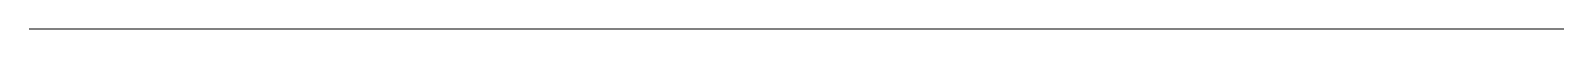
\begin{tikzpicture}
    \draw[gray,thick] (-5.5,0)--(14,0);
\end{tikzpicture}


 %%%%%%%%%%%%%%%%%%%%%%%% INICIO DEL CONTENIDO EN DOS COLUMNAS %%%%%%%%%%%%%%%%%%%%%
  
 \begin{multicols}{3}
    \begin{center}
         \LARGE{\textbf{Capítulo I: Electrostática}}\\	
         \vspace{1.2cm}
         % \Large {Lecturers Esteban Chalbaud \& Daniel Galviz} \\
         % \large{Teaching Assistant: Mauricio Gamonal \& Irvin Martínez}\\
         % \large{PhysicsLatam.com}\\
         % \vspace{1.2cm}
         \large{25 Septiembre 2025, 6:59 am (GMT-4)}\\
         % \vspace{1.2cm}
         \large{— Ficha de Trabajo —}
    \end{center}
    %%%%%%%%%%%%%%%%%%%%%%%%%%%%excercise%%%%%%%%%%%%%%%%%%%%%%%%%%%%%%%%%%%%%%%%
    \section{Capitulo noel}
Estructuralmente, Perl está basado en un estilo de bloques como los del C o AWK, y fue ampliamente adoptado por su destreza en el procesado de texto y no tener ninguna de las limitaciones de los otros lenguajes de script.La programación es el proceso de crear un conjunto de instrucciones (código) que una computadora puede ejecutar para realizar una tarea. Implica escribir, probar y mantener código en un lenguaje específico, como Python o JavaScript, para crear software y aplicaciones. La programación es fundamental para el desarrollo de la tecnología moderna, permitiendo la automatización de tareas y la creación de soluciones digitales
    \section{capitulo graciela}
Wikipedia es una enciclopedia libre,[nota 2]​ políglota y editada de manera colaborativa. Es administrada por la Fundación Wikimedia, una organización sin ánimo de lucro cuya financiación está basada en donaciones. Sus más de 63 millones de artículos en 334 idiomas han sido redactados en conjunto por voluntarios de todo el mundo,[5]​ lo que suma más de 3500 millones de ediciones, y permite que cualquier persona pueda sumarse al proyecto[6]​ para editarlos, a menos que la página se encuentre protegida contra vandalismos para evitar problemas o disputas.

Las coordenadas esféricas $(r, \theta, \varphi)$ describen la posición de un punto en el espacio mediante:

\begin{itemize}
    \item $r$: distancia del punto al origen, $r \ge 0$.
    \item $\theta$: ángulo polar, medido desde el eje $z$, $0 \le \theta \le \pi$.
    \item $\varphi$: ángulo azimutal, medido desde el eje $x$ en el plano $xy$, $0 \le \varphi < 2\pi$.
\end{itemize}

\section*{Conversión a coordenadas cartesianas}

Las relaciones entre coordenadas cartesianas $(x,y,z)$ y esféricas son:

\[
x = r \sin\theta \cos\varphi, \qquad
y = r \sin\theta \sin\varphi, \qquad
z = r \cos\theta.
\]

Las inversas son:

\[
r = \sqrt{x^2 + y^2 + z^2}, \quad
\theta = \arccos\left(\frac{z}{r}\right), \quad
\varphi = \operatorname{atan2}(y, x).
\]

\section*{Elemento de volumen}

El elemento de volumen en coordenadas esféricas se obtiene del Jacobiano:

\[
dV = r^2 \sin\theta \; dr \, d\theta \, d\varphi.
\]

\section*{Ejemplo: Volumen de una esfera}

El volumen de una esfera de radio $R$ se calcula como:

\[
V = \int_0^{2\pi}\int_0^{\pi}\int_0^R r^2 \sin\theta \; dr \, d\theta \, d\varphi
    = \frac{4}{3}\pi R^3.
\]
   


\end{multicols}
